\documentclass[11pt]{article}
\usepackage[margin=1in]{geometry}
\usepackage{amsmath,amssymb}
\usepackage{graphicx}
\usepackage{lmodern}
\usepackage[T1]{fontenc}
\usepackage{enumitem}
\usepackage{microtype}
\usepackage{tikz}
\usetikzlibrary{arrows.meta,decorations.pathreplacing}

\title{2022A F=ma Exam Review}
\author{Nathan P.}
\date{December 29, 2025}

\begin{document}
\maketitle

\section*{Problem 8}
\hspace*{\parindent} I initially thought the center-of-mass horizontal position would stay the same if it slid down, based on a frictionless problem I'd seen before. I even wrote out the math, the horizontal components of $N$ and $f$ from the box on the incline \emph{did} cancel, but it still seemed unintuitive that there would be zero friction between the incline and the ground.

The key for these statics problems is being able to treat some objects as one system. If the box and incline are treated as a single object of mass $2m$, then the internal forces do not matter, and it becomes clear that there can be no friction between the incline and the ground, because that would be an external horizontal force while the object is static.

\section*{Problem 9}
$F_v$ is the force required to keep it moving at constant $v$, meaning the net force is zero. Then
\[
2T=2mg
\]
since the mass is doubled, so
\[
T=F_v=mg
\]

However, when it comes to acceleration, the mass accelerates upward at half the acceleration with which the string is pulled, due to conservation of string (two strings supporting the mass, so pulling up by $x$ means the mass moves up by $x/2$ since we need to split string length between the two sides).

Thus,
\[
2T-2mg=2m\left(\frac{a}{2}\right)
\]
\[
T=mg+\frac{ma}{2}
\]
which is less than the result one might initially expect.

\section*{Problem 11}
\hspace*{\parindent} The underlying idea was correct: getting to the midway point is essentially the finish line, because once that point is crossed, the second planet's gravitational force takes over.

A helpful way to picture it is that the midpoint is the threshold. If the rocket can make it to that point, then it can cross, because beyond the midpoint the second planet pulls more strongly.

\begin{center}
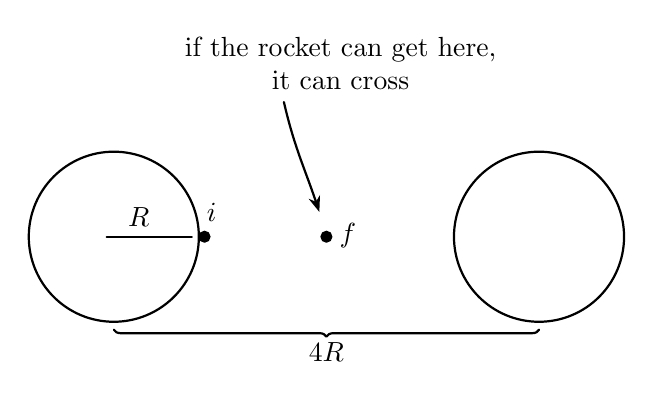
\begin{tikzpicture}[scale=0.9, line cap=round, line join=round, >={Stealth[length=2mm]}]
    \draw[thick] (0,0) circle (1.2);
    \draw[thick] (6,0) circle (1.2);

    \draw[thick] (-0.1,0) -- (1.1,0);
    \node[above] at (0.35,0) {$R$};

    \filldraw[black] (1.28,0) circle (2.2pt);
    \filldraw[black] (3,0) circle (2.2pt);

    \node[above] at (1.38,0.08) {$i$};
    \node[right] at (3.05,0.02) {$f$};

    \draw[decorate,decoration={brace,mirror,raise=8pt},thick] (0,-1) -- (6,-1);
    \node[below] at (3,-1.35) {$4R$};

    \draw[->,thick] (2.4,1.9) .. controls (2.55,1.25) and (2.7,0.95) .. (2.9,0.35);
    \node[align=center] at (3.2,2.45) {if the rocket can get here,\\ it can cross};
\end{tikzpicture}
\end{center}

The incorrect step was ignoring gravitational potential from the second planet and only setting the initial $U_G+K_i$ equal to the final gravitational potential from the first planet. However, gravity from the second planet always exists, so its contribution to the potential energy must be included throughout.

\section*{Problem 12}
The radial acceleration of the pulley is related to the linear acceleration of the mass by
\[
a=r\alpha
\]
The right mass has radius $2r$, so its linear acceleration is $2a$, which leads correspondingly to $2F$.

More generally, when a problem says ``concentric'' or ``attached'' or something similar, that is a cue that the objects rotate together unless stated otherwise. That makes it possible to relate their accelerations through $a=r\alpha$.

\section*{Problem 13}
\hspace*{\parindent} To clarify, ``in the plane of the page'' means the force lies in the page so that it is fully visible on the page; it does \emph{not} mean into or perpendicular to the page.

The applied force must also be perpendicular to the relevant lever arm because the question asks for the minimum force. A perpendicular force produces the maximum torque, whereas a horizontal force here would be applied at an angle.

From there, balance the clockwise and counterclockwise torques.

\section*{Problem 14}
\hspace*{\parindent} The magnitude of the vertical velocity decreases because there is an increasing upward normal-force component from the bowl. A useful strategy here is to compare the initial and final states and recognize that the vertical velocity starts and ends at zero.

To verify whether the speed decreases, use energy. The object never gains potential energy, so the speed never decreases.

To verify whether the horizontal or vertical velocity ever decreases, check whether there is ever a force opposing that component of the velocity. Horizontally, no: there is only a rightward component of normal force, so the block only speeds up to the right during this interval. Vertically, there is an upward normal-force component, so it makes sense that the vertical motion slows down.

\section*{Problem 15}
\hspace*{\parindent} This problem was meant to be solved with limiting cases. It is often worth trying limiting cases when variables like $v$, $g$, $d$, or $h$ appear, when the math looks as though it is going to become messy but the answer choices differ in important ways, or when the problem involves optimization.

Consider what happens when $v$, $g$, or $d$ go to $0$ or to infinity. Particularly, the case
\[
d_{\max}=\frac{v^2}{g}
\]
for which $\theta$ would have to be $45^\circ$.

\section*{Problem 16}
Balance torques for this statics problem with triangle geometry.

\begin{center}
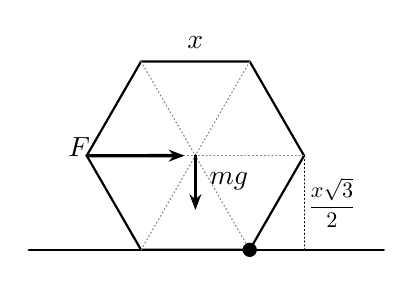
\begin{tikzpicture}[scale=0.92, line cap=round, line join=round, >={Stealth[length=2mm]}]
    \draw[thick] (-2.3,0) -- (2.6,0);

    \coordinate (L)  at (-1.5,1.30);
    \coordinate (UL) at (-0.75,2.60);
    \coordinate (UR) at (0.75,2.60);
    \coordinate (R)  at (1.5,1.30);
    \coordinate (LR) at (0.75,0);
    \coordinate (LL) at (-0.75,0);
    \coordinate (C)  at (0,1.30);
    \coordinate (P)  at (0.75,0);

    \draw[thick] (L) -- (UL) -- (UR) -- (R) -- (LR) -- (LL) -- cycle;

    \draw[densely dotted, gray] (L) -- (C);
    \draw[densely dotted, gray] (UL) -- (C);
    \draw[densely dotted, gray] (UR) -- (C);
    \draw[densely dotted, gray] (R) -- (C);
    \draw[densely dotted, gray] (LL) -- (C);
    \draw[densely dotted, gray] (LR) -- (C);

    \fill (P) circle (2.8pt);

    \draw[->, very thick] (L) -- (-0.15,1.30);
    \node[left] at (-1.32,1.42) {$F$};

    \draw[->, very thick] (C) -- (0,0.55);
    \node[right] at (0.06,0.95) {$mg$};

    \node[above] at (0,2.64) {$x$};

    \draw[densely dotted] (1.5,0) -- (1.5,1.30);
    \node[scale=0.8, right] at (1.45,0.65) {$\dfrac{x\sqrt{3}}{2}$};
\end{tikzpicture}
\end{center}

\section*{Problem 17}
Use the definition of center of mass:
\[
m_1d_1=m_2d_2
\]
In general, $m_1\neq m_2$.

The remaining point of confusion is why $I_1\neq I_2$; that distinction should be checked carefully from the geometry and mass distribution rather than assumed from the center-of-mass relation alone.

\section*{Problem 19}
\[
P_{\text{hydro}}=F_{\text{buoy}}-\rho gh
\]

\section*{Problem 21}
The height of the cork is determined by the buoyant force on it, with
\[
F_{\text{buoy}}=mg
\]
When the system is accelerating, the right idea is to think in terms of an effective gravitational field, $g_{\text{eff}}$. However, all weights are modified in the same way, so the relation
\[
\rho V_{\text{sub}}g=mg
\]
does not change in form.

\section*{Problem 22}
The main steps here are:

\begin{itemize}[leftmargin=1.5em]
    \item Sum forces in the directions of motion
    \item Use symmetry: pick one symmetric object to focus on
    \item Use the motion dependence: the angle stays the same throughout the motion
    \item Careful with angles
    \item Write $\sum F_y$ and $\sum F_x$ in the directions of motion; $N$ is unknown, so sub that in $\sum F_y$

    \item Often the motion dependence can be found through $\tan\theta=\frac{x}{y}$.
\end{itemize}
\section*{Problem 23}
We know the time in the air depends only on the vertical velocity.

\noindent For linear drag, yes, the components are independent because
\[
v\sin\theta=v\cdot \frac{v_y}{v}=v_y
\]
which is independent of
\[
v_x=v\cos\theta
\]

\noindent However, the geometry for quadratic drag is different:
\[
F_{\text{drag},y}=bv^2\cos\theta=bv^2\frac{v_y}{v}=bv_y\sqrt{v_x^2+v_y^2}
\]
As this expression shows, the drag depends on $v_x$, so the time to fall would be longer.

\section*{Problem 25}
\noindent
\begin{minipage}[t]{0.7\textwidth}
Consider a small piece $dm$. For small angles,
\[
\sin\theta\approx \theta
\]
Then
\[
\mu T\theta=mg.
\]

Assuming uniform density, the ratio of a small mass element to a small angle is the same as that of the whole object to the full circle:
\[
\frac{dm}{d\theta}=\frac{m}{2\pi}
\]
\end{minipage}\hfill
\begin{minipage}[t]{0.25\textwidth}
\vspace{0pt}
\centering
\includegraphics[width=\textwidth]{assets/problem25-sketch.png}
\end{minipage}

\end{document}